\subsection{Servo}

The Servo recieves a PWM signal by 3 wires: power, ground, and signal, connected to a 5V pin of the arduino. The period time recieved is converted into an angle by the servo to control the steering of the tracks as seen on \figref{timeVSangle}. An angle of 90° is the normal position for going straight ahead.\\

A mechanical arm is mounted on the servo and connected to the brakes of the tracks. When the servo rotates one way, it triggers more or less the brakes on the left or right side according to the value of the angle sent.\\

For steering the direction of the vehicle, the motor does not need to be revised. When one track brakes, it forces the vehicle to turn this way, and the other track turns faster for having a better bend thanks to the differential gears.\\\\

%source http://www.societyofrobots.com/actuators_servos.shtml\\

\begin{figure}[H]
	\centering
	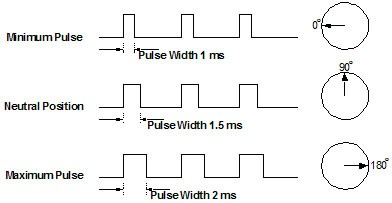
\includegraphics[scale=1]{figures/timeVSangle.jpg}
	\caption{Convertion from time to angle by the servo\cite {AServos}}
	\label{timeVSangle}
\end{figure}
\todo{insert source}
